\newpage
\phantomsection %实现目录的正确跳转
\section*{\hei\large 蟠桃会~\protect\footnote{此戏别名《海屋添筹》或《八仙庆寿》,是一出武旦戏。}~%\protect\hyperlink{fn632}{\textsuperscript{632}}
{\small 之}~吕洞宾$^{\ast}$}
\addcontentsline{toc}{section}{\hei 蟠桃会~{\small 之}~吕洞宾}

\hangafter=1                   %2. 设置从第1⾏之后开始悬挂缩进  %
\setlength{\parindent}{0pt}{
{\centerline{{{[}\hei 第一场{]}}}}
\vspace{5pt}

\setlength{\hangindent}{56pt}{【{\akai 西皮原板}】忆昔当年赴科场,科场中提笔做文章。文章幸喜龙颜赏,赏赐我进士伴君王。陪王伴君心不想,一心只想上天堂。天堂就在瑶池上\footnote{此句吴小如先生从刘曾复先生学的是``天堂远在瑶池上''。}%\protect\hyperlink{fn633}{\textsuperscript{633}}
,瑶池以上福寿绵长。}

\vspace{3pt}{\centerline{{{[}{\hei 第二场}{]}}}}\vspace{5pt}

{【{\akai 西皮散板}】离了洞府到仙界,见了众仙说开怀。}

{【{\akai 西皮散板}】瑶池以上寿筵席开。}

\setlength{\hangindent}{56pt}{{【{\akai 西皮原板}】今日里饮酒多爽快,好似仙子({\akai 或}:~好一似黄粱)赴瑶台。这仙女({\akai 或}:~这仙子)生得呀多娇态,眉清目秀送情来。趁此佳兴({\akai 或}:~趁此酒兴)破了戒,}
}

{【{\akai 西皮原板}】众仙道我理不该。将身且坐({\akai 或}:~将身来在)瑶池外,昏昏沉沉睡石台。}

\vspace{3pt}{\centerline{{{[}{\hei 第三场}{]}}}}\vspace{5pt}

{【{\akai 西皮导板}】沉醉东风}\footnote{樊剑{\scriptsize 君}此处建议作``沉醉洞府''。}%\protect\hyperlink{fn634}{\textsuperscript{634}}
{月儿高,}

\setlength{\hangindent}{56pt}{{【{\akai 西皮原板}】忆昔当初饮酕醄。两足徘徊任颠倒,湘子、仙姑发笑嘲。你道我当真吃醉了,任意随心乐逍遥。游戏三昧多奥妙,}
}

\setlength{\hangindent}{56pt}{【{\akai 西皮快板}】坎离\footnote{八卦中
``坎''(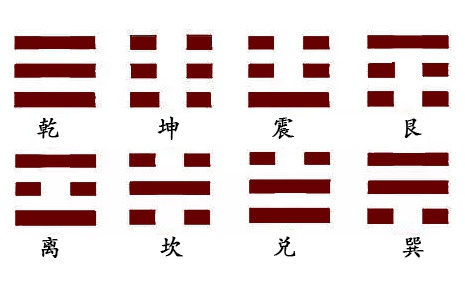
\includegraphics[height=10pt,width=10pt, viewport=120 59 225 140,clip]{Eight_Gua.jpeg})为水,
``离''(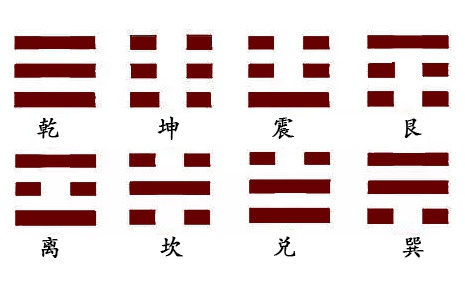
\includegraphics[height=10pt,width=10pt, viewport=5 59 100 140,clip]{Eight_Gua.jpeg})为火。此处寓为``水火既济''之意。}%\protect\hyperlink{fn635}{\textsuperscript{635}}
二字本相调。不觉来到东海道,海水接天浪滔滔。}

{【{\akai 西皮散板}】宝剑扔在东海道,你看我醉仙家的道法高不高?}

{【{\akai 西皮散板}】柳仙带路东海道,万丈波涛走一遭。}

{【{\akai 西皮散板}】湘子说话不中听,丢了宝贝你问旁人。}

{【{\akai 西皮散板}】洞宾主意拿得稳,从今后不管闲事情。}

(李铁拐\hspace{20pt}【{\akai 西皮散板}】$\cdots${}$\cdots${}{入东海道,)}

{【{\akai 西皮散板}】从今后戒酒最为高。}
}
